\documentclass[twoside]{book}

% Packages required by doxygen
\usepackage{fixltx2e}
\usepackage{calc}
\usepackage{doxygen}
\usepackage[export]{adjustbox} % also loads graphicx
\usepackage{graphicx}
\usepackage[utf8]{inputenc}
\usepackage{makeidx}
\usepackage{multicol}
\usepackage{multirow}
\PassOptionsToPackage{warn}{textcomp}
\usepackage{textcomp}
\usepackage[nointegrals]{wasysym}
\usepackage[table]{xcolor}

% Font selection
\usepackage[T1]{fontenc}
\usepackage[scaled=.90]{helvet}
\usepackage{courier}
\usepackage{amssymb}
\usepackage{sectsty}
\renewcommand{\familydefault}{\sfdefault}
\allsectionsfont{%
  \fontseries{bc}\selectfont%
  \color{darkgray}%
}
\renewcommand{\DoxyLabelFont}{%
  \fontseries{bc}\selectfont%
  \color{darkgray}%
}
\newcommand{\+}{\discretionary{\mbox{\scriptsize$\hookleftarrow$}}{}{}}

% Page & text layout
\usepackage{geometry}
\geometry{%
  a4paper,%
  top=2.5cm,%
  bottom=2.5cm,%
  left=2.5cm,%
  right=2.5cm%
}
\tolerance=750
\hfuzz=15pt
\hbadness=750
\setlength{\emergencystretch}{15pt}
\setlength{\parindent}{0cm}
\setlength{\parskip}{3ex plus 2ex minus 2ex}
\makeatletter
\renewcommand{\paragraph}{%
  \@startsection{paragraph}{4}{0ex}{-1.0ex}{1.0ex}{%
    \normalfont\normalsize\bfseries\SS@parafont%
  }%
}
\renewcommand{\subparagraph}{%
  \@startsection{subparagraph}{5}{0ex}{-1.0ex}{1.0ex}{%
    \normalfont\normalsize\bfseries\SS@subparafont%
  }%
}
\makeatother

% Headers & footers
\usepackage{fancyhdr}
\pagestyle{fancyplain}
\fancyhead[LE]{\fancyplain{}{\bfseries\thepage}}
\fancyhead[CE]{\fancyplain{}{}}
\fancyhead[RE]{\fancyplain{}{\bfseries\leftmark}}
\fancyhead[LO]{\fancyplain{}{\bfseries\rightmark}}
\fancyhead[CO]{\fancyplain{}{}}
\fancyhead[RO]{\fancyplain{}{\bfseries\thepage}}
\fancyfoot[LE]{\fancyplain{}{}}
\fancyfoot[CE]{\fancyplain{}{}}
\fancyfoot[RE]{\fancyplain{}{\bfseries\scriptsize Generated by Doxygen }}
\fancyfoot[LO]{\fancyplain{}{\bfseries\scriptsize Generated by Doxygen }}
\fancyfoot[CO]{\fancyplain{}{}}
\fancyfoot[RO]{\fancyplain{}{}}
\renewcommand{\footrulewidth}{0.4pt}
\renewcommand{\chaptermark}[1]{%
  \markboth{#1}{}%
}
\renewcommand{\sectionmark}[1]{%
  \markright{\thesection\ #1}%
}

% Indices & bibliography
\usepackage{natbib}
\usepackage[titles]{tocloft}
\setcounter{tocdepth}{3}
\setcounter{secnumdepth}{5}
\makeindex

% Custom commands
\newcommand{\clearemptydoublepage}{%
  \newpage{\pagestyle{empty}\cleardoublepage}%
}

\usepackage{caption}
\captionsetup{labelsep=space,justification=centering,font={bf},singlelinecheck=off,skip=4pt,position=top}

%===== C O N T E N T S =====

\begin{document}

% Titlepage & ToC
\pagenumbering{alph}
\begin{titlepage}
\vspace*{7cm}
\begin{center}%
{\Large Software documentation -\/ Command-\/line tools }\\
\vspace*{1cm}
{\large Generated by Doxygen 1.8.13}\\
\end{center}
\end{titlepage}
\clearemptydoublepage
\pagenumbering{roman}
\tableofcontents
\clearemptydoublepage
\pagenumbering{arabic}

%--- Begin generated contents ---
\chapter{Command line tools}
\label{index}Those functions allows to use the board through a serial port\begin{DoxyAuthor}{Author}
{\itshape Centro \char`\"{}\+E.\+Piaggio\char`\"{}} 
\end{DoxyAuthor}
\begin{DoxyCopyright}{Copyright}
(C) 2012-\/2016 qbrobotics. All rights reserved. 

(C) 2017 Centro \char`\"{}\+E.\+Piaggio\char`\"{}. All rights reserved.
\end{DoxyCopyright}
\begin{DoxyDate}{Date}
October 01, 2017
\end{DoxyDate}
This is a set of functions that allows to use the boards via a serial port.

Those A\+P\+Is can be compiled for Unix systems like Linux and Mac OS X and even for Windows. Refer to {\tt https\+://github.\+com/\+N\+M\+M\+I/qb\+A\+P\+I/tree/centropiaggio} for detailed instructions. 
\chapter{Data Structure Index}
\section{Data Structures}
Here are the data structures with brief descriptions\+:\begin{DoxyCompactList}
\item\contentsline{section}{\textbf{ global\+\_\+args} }{\pageref{structglobal__args}}{}
\item\contentsline{section}{\textbf{ global\+\_\+var} }{\pageref{structglobal__var}}{}
\item\contentsline{section}{\textbf{ position} }{\pageref{structposition}}{}
\end{DoxyCompactList}

\chapter{File Index}
\section{File List}
Here is a list of all documented files with brief descriptions\+:\begin{DoxyCompactList}
\item\contentsline{section}{\textbf{ definitions.\+h} \\*Definitions for board commands, parameters and packages }{\pageref{definitions_8h}}{}
\item\contentsline{section}{\textbf{ hand\+\_\+demo.\+c} \\*Demonstration file }{\pageref{hand__demo_8c}}{}
\item\contentsline{section}{\textbf{ qbadmin.\+c} \\*Command line tools file }{\pageref{qbadmin_8c}}{}
\item\contentsline{section}{\textbf{ qbmove\+\_\+backup.\+c} \\*Command line tools file }{\pageref{qbmove__backup_8c}}{}
\item\contentsline{section}{\textbf{ qbmove\+\_\+init.\+c} \\*Command line tools file }{\pageref{qbmove__init_8c}}{}
\item\contentsline{section}{\textbf{ qbmove\+\_\+pos\+\_\+stiff\+\_\+demo.\+c} \\*Command line tools file }{\pageref{qbmove__pos__stiff__demo_8c}}{}
\item\contentsline{section}{\textbf{ qbmove\+\_\+test.\+c} \\*Command line tools file }{\pageref{qbmove__test_8c}}{}
\item\contentsline{section}{\textbf{ qbparam.\+c} \\*Command line tools file }{\pageref{qbparam_8c}}{}
\end{DoxyCompactList}

\chapter{Data Structure Documentation}
\section{global\+\_\+args Struct Reference}
\label{structglobal__args}\index{global\+\_\+args@{global\+\_\+args}}
\subsection*{Data Fields}
\begin{DoxyCompactItemize}
\item 
\mbox{\label{structglobal__args_accfd0301c469314772cc651ec198d492}} 
int {\bfseries device\+\_\+id}
\item 
\mbox{\label{structglobal__args_a8c2bd6bbe7e544186ac9dafe368eda0a}} 
int \textbf{ flag\+\_\+set\+\_\+inputs}
\begin{DoxyCompactList}\small\item\em ./qbadmin -\/s option \end{DoxyCompactList}\item 
\mbox{\label{structglobal__args_ae6be84e61dfa72e2992e18b2ff872d37}} 
int \textbf{ flag\+\_\+get\+\_\+measurements}
\begin{DoxyCompactList}\small\item\em ./qbadmin -\/g option \end{DoxyCompactList}\item 
\mbox{\label{structglobal__args_a357acdae444e13e67d3747246a2a6537}} 
int \textbf{ flag\+\_\+activate}
\begin{DoxyCompactList}\small\item\em ./qbadmin -\/a option \end{DoxyCompactList}\item 
\mbox{\label{structglobal__args_a3f8a32491b8271e7dcf9645888fd5d90}} 
int \textbf{ flag\+\_\+deactivate}
\begin{DoxyCompactList}\small\item\em ./qbadmin -\/d option \end{DoxyCompactList}\item 
\mbox{\label{structglobal__args_a666e67d4cbdc4b0c0ceaebc7f0d7e4ae}} 
int \textbf{ flag\+\_\+ping}
\begin{DoxyCompactList}\small\item\em ./qbadmin -\/p option \end{DoxyCompactList}\item 
\mbox{\label{structglobal__args_a5d91f73cfac19063f3b690444214cb11}} 
int \textbf{ flag\+\_\+serial\+\_\+port}
\begin{DoxyCompactList}\small\item\em ./qbadmin -\/t option \end{DoxyCompactList}\item 
\mbox{\label{structglobal__args_a2d410324c656ed3cf62239ef07f19df6}} 
int \textbf{ flag\+\_\+verbose}
\begin{DoxyCompactList}\small\item\em ./qbadmin -\/v option \end{DoxyCompactList}\item 
\mbox{\label{structglobal__args_afc413e6af53fa6f9942e91061ec9b1f7}} 
int \textbf{ flag\+\_\+file}
\begin{DoxyCompactList}\small\item\em ./qbadmin -\/f option \end{DoxyCompactList}\item 
\mbox{\label{structglobal__args_a86b9e5670875a9a7e17f30b62e988d89}} 
int \textbf{ flag\+\_\+log}
\begin{DoxyCompactList}\small\item\em ./qbadmin -\/l option \end{DoxyCompactList}\item 
\mbox{\label{structglobal__args_a1e27bdb894b1a7eb6221b1bd463dc71d}} 
int \textbf{ flag\+\_\+get\+\_\+emg}
\begin{DoxyCompactList}\small\item\em ./qbadmin -\/q option to get the E\+MG sensors measurements \end{DoxyCompactList}\item 
\mbox{\label{structglobal__args_a66d5c9e9750727f229d685d9399218d0}} 
int \textbf{ flag\+\_\+set\+\_\+zeros}
\begin{DoxyCompactList}\small\item\em ./qbadmin -\/z option \end{DoxyCompactList}\item 
\mbox{\label{structglobal__args_a976efe8621136ad8b129e72d53be6705}} 
int \textbf{ flag\+\_\+use\+\_\+gen\+\_\+sin}
\begin{DoxyCompactList}\small\item\em ./qbadmin -\/y option \end{DoxyCompactList}\item 
\mbox{\label{structglobal__args_ada343d7375a97b92b74f21ff14998520}} 
int \textbf{ flag\+\_\+calibration}
\begin{DoxyCompactList}\small\item\em ./qbadmin -\/k option to start a series of hand closures and openings \end{DoxyCompactList}\item 
\mbox{\label{structglobal__args_a884582f66057291a6a1f030d5d46d9d5}} 
int \textbf{ flag\+\_\+get\+\_\+currents}
\begin{DoxyCompactList}\small\item\em ./qbadmin -\/c option \end{DoxyCompactList}\item 
\mbox{\label{structglobal__args_a8488439bc3473b5fb08964d06b51b80a}} 
int \textbf{ flag\+\_\+bootloader\+\_\+mode}
\begin{DoxyCompactList}\small\item\em ./qbadmin -\/b option \end{DoxyCompactList}\item 
\mbox{\label{structglobal__args_ac814e1ddd60d50ef7e0aeac6a5ea38b0}} 
int \textbf{ flag\+\_\+set\+\_\+pos\+\_\+stiff}
\begin{DoxyCompactList}\small\item\em ./qbadmin -\/e option \end{DoxyCompactList}\item 
\mbox{\label{structglobal__args_aa9b8d91302ac6dbb99023c9363c352f8}} 
int \textbf{ flag\+\_\+get\+\_\+velocities}
\begin{DoxyCompactList}\small\item\em ./qbadmin -\/i option \end{DoxyCompactList}\item 
\mbox{\label{structglobal__args_af72013af180143fd3cce334fca450bec}} 
int \textbf{ flag\+\_\+get\+\_\+accelerations}
\begin{DoxyCompactList}\small\item\em ./qbadmin -\/o option \end{DoxyCompactList}\item 
\mbox{\label{structglobal__args_a8bae74d00a58818ba0dad8bc3fb46625}} 
int \textbf{ flag\+\_\+set\+\_\+cuff\+\_\+inputs}
\begin{DoxyCompactList}\small\item\em ./qbadmin -\/u option \end{DoxyCompactList}\item 
\mbox{\label{structglobal__args_aeb7e77450221e7de1da5ae0701a8c7af}} 
int \textbf{ flag\+\_\+set\+\_\+baudrate}
\begin{DoxyCompactList}\small\item\em ./qbadmin -\/R option \end{DoxyCompactList}\item 
\mbox{\label{structglobal__args_a5416bb93d203c57a7fc6fe93957f5c14}} 
int \textbf{ flag\+\_\+set\+\_\+watchdog}
\begin{DoxyCompactList}\small\item\em ./qbadmin -\/W option \end{DoxyCompactList}\item 
\mbox{\label{structglobal__args_ab4fab167b07a819ebd9cdff9d9c232b0}} 
int \textbf{ flag\+\_\+polling}
\begin{DoxyCompactList}\small\item\em ./qbadmin -\/P option \end{DoxyCompactList}\item 
\mbox{\label{structglobal__args_a9781d8e86f2d0d0414d313fec085d20e}} 
int \textbf{ flag\+\_\+baudrate}
\begin{DoxyCompactList}\small\item\em ./qbadmin -\/B option \end{DoxyCompactList}\item 
\mbox{\label{structglobal__args_a58c1425e6d892db3e470cdd99529fce0}} 
int \textbf{ flag\+\_\+get\+\_\+joystick}
\begin{DoxyCompactList}\small\item\em ./qbadmin -\/j option \end{DoxyCompactList}\item 
\mbox{\label{structglobal__args_a5cc1e4efdeddb5e75d5e733f00e5087f}} 
int \textbf{ flag\+\_\+ext\+\_\+drive}
\begin{DoxyCompactList}\small\item\em ./qbadmin -\/x option \end{DoxyCompactList}\item 
\mbox{\label{structglobal__args_a5c5d83977377b63e3671b52680be11aa}} 
short int {\bfseries inputs} [N\+U\+M\+\_\+\+O\+F\+\_\+\+M\+O\+T\+O\+RS]
\item 
\mbox{\label{structglobal__args_a4c65d251aa919a9ae56d11639a748ccf}} 
short int {\bfseries measurements} [4]
\item 
\mbox{\label{structglobal__args_aa064f75f1bb48d252dabea993cd8c393}} 
short int {\bfseries velocities} [4]
\item 
\mbox{\label{structglobal__args_a6fe131122f89735be8fb030f8333e8c8}} 
short int {\bfseries accelerations} [4]
\item 
\mbox{\label{structglobal__args_a8e63e8b1dcf1ee3b6429110e26a7ef3d}} 
short int {\bfseries measurement\+\_\+offset} [4]
\item 
\mbox{\label{structglobal__args_aff0783d0bf2ae80eadc0c85a84db1549}} 
short int {\bfseries currents} [N\+U\+M\+\_\+\+O\+F\+\_\+\+M\+O\+T\+O\+RS]
\item 
\mbox{\label{structglobal__args_a522de19291f23fb0be3eb346cc1957e9}} 
char {\bfseries filename} [255]
\item 
\mbox{\label{structglobal__args_ad0345d4821606480fcb0e28327340660}} 
char {\bfseries log\+\_\+file} [255]
\item 
\mbox{\label{structglobal__args_a74aee2224894f2773538b376bcdd3a65}} 
short int \textbf{ calib\+\_\+speed}
\begin{DoxyCompactList}\small\item\em Calibration speed. \end{DoxyCompactList}\item 
\mbox{\label{structglobal__args_a97358fe57110982e565254fa7310cf8f}} 
short int \textbf{ calib\+\_\+repetitions}
\begin{DoxyCompactList}\small\item\em Calibration repetitions. \end{DoxyCompactList}\item 
\mbox{\label{structglobal__args_ac99613e9febb46b081ae696a20e34c62}} 
short int \textbf{ emg} [N\+U\+M\+\_\+\+O\+F\+\_\+\+E\+M\+GS]
\begin{DoxyCompactList}\small\item\em Emg sensors values read from the device. \end{DoxyCompactList}\item 
\mbox{\label{structglobal__args_a0cace64ae2459f06bc0bda1979b0c06f}} 
short int \textbf{ joystick} [2]
\begin{DoxyCompactList}\small\item\em Analog joystick measurements. \end{DoxyCompactList}\item 
\mbox{\label{structglobal__args_af848f8d2dca8dfbccc182293c8ba25bf}} 
short int {\bfseries ext\+\_\+drive}
\item 
\mbox{\label{structglobal__args_a8f68c2db71004b2beac47c7ce6feb94c}} 
short int {\bfseries Baud\+Rate}
\item 
\mbox{\label{structglobal__args_a15a8bc4e37e5294ee939c1dd620095a8}} 
int {\bfseries save\+\_\+baurate}
\item 
\mbox{\label{structglobal__args_abd2a5fb7d2e58a98c4394067565b5492}} 
short int {\bfseries W\+DT}
\item 
\mbox{\label{structglobal__args_ac3ca959d3b7ae254f86531e0b82affcb}} 
F\+I\+LE $\ast$ {\bfseries emg\+\_\+file}
\item 
\mbox{\label{structglobal__args_a5fbba9db8f8d479d7607ec6e8617026a}} 
F\+I\+LE $\ast$ {\bfseries log\+\_\+file\+\_\+fd}
\end{DoxyCompactItemize}


The documentation for this struct was generated from the following file\+:\begin{DoxyCompactItemize}
\item 
\textbf{ qbadmin.\+c}\end{DoxyCompactItemize}

\section{global\+\_\+var Struct Reference}
\label{structglobal__var}\index{global\+\_\+var@{global\+\_\+var}}
\subsection*{Data Fields}
\begin{DoxyCompactItemize}
\item 
\mbox{\label{structglobal__var_a085c28d6493b324a90e58ea1b9f0c9e2}} 
int {\bfseries flag\+\_\+set\+\_\+time}
\item 
\mbox{\label{structglobal__var_a9e8101269e0ff94ba2ec010275363894}} 
int {\bfseries flag\+\_\+set\+\_\+repetitions}
\end{DoxyCompactItemize}


The documentation for this struct was generated from the following file\+:\begin{DoxyCompactItemize}
\item 
\textbf{ qbmove\+\_\+test.\+c}\end{DoxyCompactItemize}

\section{position Struct Reference}
\label{structposition}\index{position@{position}}
\subsection*{Data Fields}
\begin{DoxyCompactItemize}
\item 
\mbox{\label{structposition_a3f6abbd70f28831ca50df1deece62d27}} 
float {\bfseries prec}
\item 
\mbox{\label{structposition_acd65ff39e6ad988e189dc854d5ede11b}} 
float {\bfseries act}
\end{DoxyCompactItemize}


The documentation for this struct was generated from the following file\+:\begin{DoxyCompactItemize}
\item 
\textbf{ qbadmin.\+c}\end{DoxyCompactItemize}

\chapter{File Documentation}
\section{definitions.\+h File Reference}
\label{definitions_8h}\index{definitions.\+h@{definitions.\+h}}


Definitions for board commands, parameters and packages.  


{\ttfamily \#include $<$math.\+h$>$}\newline
Include dependency graph for definitions.\+h\+:\nopagebreak
\begin{figure}[H]
\begin{center}
\leavevmode
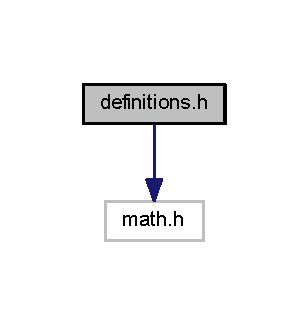
\includegraphics[width=148pt]{definitions_8h__incl}
\end{center}
\end{figure}
This graph shows which files directly or indirectly include this file\+:\nopagebreak
\begin{figure}[H]
\begin{center}
\leavevmode
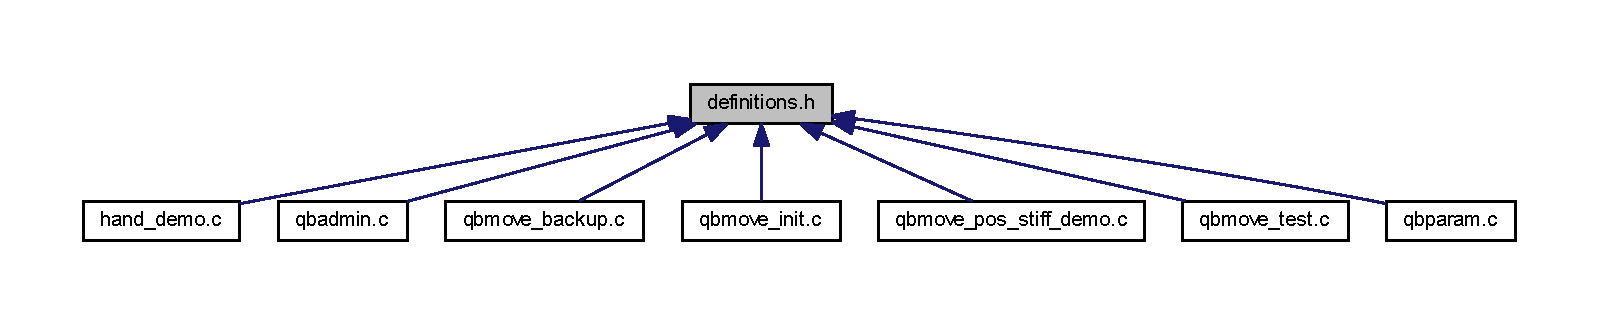
\includegraphics[width=350pt]{definitions_8h__dep__incl}
\end{center}
\end{figure}
\subsection*{Macros}
\begin{DoxyCompactItemize}
\item 
\mbox{\label{definitions_8h_a82178bde559e31158313c53e55709f7b}} 
\#define {\bfseries Q\+B\+A\+D\+M\+I\+N\+\_\+\+V\+E\+R\+S\+I\+ON}~\char`\"{}v6.\+1.\+0\char`\"{}
\item 
\mbox{\label{definitions_8h_a39ac50737c1ee7d5b723b2597fdf6f26}} 
\#define {\bfseries N\+U\+M\+\_\+\+O\+F\+\_\+\+M\+O\+T\+O\+RS}~2
\item 
\mbox{\label{definitions_8h_a8e55cba7b8d4f9aa1eb36f311ce121e5}} 
\#define {\bfseries N\+U\+M\+\_\+\+O\+F\+\_\+\+E\+M\+GS}~2
\item 
\mbox{\label{definitions_8h_a598a3330b3c21701223ee0ca14316eca}} 
\#define {\bfseries PI}~3.\+14159265359
\item 
\mbox{\label{definitions_8h_a2674041fcb6b33ea03b7441c5bf07da1}} 
\#define {\bfseries D\+E\+F\+A\+U\+L\+T\+\_\+\+R\+E\+S\+O\+L\+U\+T\+I\+ON}~1
\item 
\mbox{\label{definitions_8h_a9df8ee92f567229e4e969a89792f7909}} 
\#define {\bfseries D\+E\+F\+A\+U\+L\+T\+\_\+\+I\+N\+F\+\_\+\+L\+I\+M\+IT}~-\/15000
\item 
\mbox{\label{definitions_8h_a664de08cc70be246edd326c4832574bb}} 
\#define {\bfseries D\+E\+F\+A\+U\+L\+T\+\_\+\+S\+U\+P\+\_\+\+L\+I\+M\+IT}~15000
\item 
\mbox{\label{definitions_8h_ab9fe47395310b34fa1ceb112c9ca10e2}} 
\#define {\bfseries B\+R\+O\+A\+D\+C\+A\+S\+T\+\_\+\+ID}~0
\item 
\mbox{\label{definitions_8h_a4c6daad09923a0ab3ed52ebb1c0b8cb8}} 
\#define {\bfseries D\+E\+F\+A\+U\+L\+T\+\_\+\+P\+I\+D\+\_\+P}~0.\+1
\item 
\mbox{\label{definitions_8h_a6f7a63a5d40ee41381abe79b78993567}} 
\#define {\bfseries D\+E\+F\+A\+U\+L\+T\+\_\+\+P\+I\+D\+\_\+I}~0
\item 
\mbox{\label{definitions_8h_ab285c4cd42477c9669f9981d03572d2f}} 
\#define {\bfseries D\+E\+F\+A\+U\+L\+T\+\_\+\+P\+I\+D\+\_\+D}~0.\+8
\item 
\mbox{\label{definitions_8h_a4956377066b3b3074de9c79d7e1d8967}} 
\#define {\bfseries D\+E\+F\+A\+U\+L\+T\+\_\+\+I\+N\+C\+R\+E\+M\+E\+NT}~1
\item 
\mbox{\label{definitions_8h_a8c5790f774337ec087041124dda03ed4}} 
\#define {\bfseries D\+E\+F\+A\+U\+L\+T\+\_\+\+S\+T\+I\+F\+F\+N\+E\+SS}~30
\item 
\mbox{\label{definitions_8h_a92f641bf6a2b5f3e0277d62d29158bff}} 
\#define {\bfseries D\+E\+F\+A\+U\+L\+T\+\_\+\+M\+A\+X\+\_\+\+E\+X\+C\+U\+R\+S\+I\+ON}~330
\item 
\mbox{\label{definitions_8h_ac328e551bde3d39b6d7b8cc9e048d941}} 
\#define {\bfseries Z\+E\+RO}~0
\item 
\mbox{\label{definitions_8h_a2719be2b85fcfd6fd26291a9a7775ea7}} 
\#define {\bfseries M\+A\+X\+\_\+\+F\+O\+R\+W\+A\+R\+D\+\_\+\+S\+T\+I\+F\+F\+N\+E\+SS}~32767
\item 
\mbox{\label{definitions_8h_ad91fa28a852c573709249b16fca30d23}} 
\#define {\bfseries M\+A\+X\+\_\+\+R\+E\+V\+E\+R\+S\+E\+\_\+\+S\+T\+I\+F\+F\+N\+E\+SS}~-\/32768
\item 
\mbox{\label{definitions_8h_adc098850cdde5fbe8e5f4fe910f9ce27}} 
\#define {\bfseries D\+E\+G\+\_\+\+T\+I\+C\+K\+\_\+\+M\+U\+L\+T\+I\+P\+L\+I\+ER}~(65536.\+0 / (360.\+0 $\ast$ (pow(2, D\+E\+F\+A\+U\+L\+T\+\_\+\+R\+E\+S\+O\+L\+U\+T\+I\+ON))))
\item 
\mbox{\label{definitions_8h_a44483e681594d0e510fd59c2b4b09ed9}} 
\#define {\bfseries B\+A\+U\+D\+\_\+\+R\+A\+T\+E\+\_\+\+T\+\_\+2000000}~0
\item 
\mbox{\label{definitions_8h_ad2c3e3edb0886633d686996e2f8c48e6}} 
\#define {\bfseries B\+A\+U\+D\+\_\+\+R\+A\+T\+E\+\_\+\+T\+\_\+460800}~1
\item 
\mbox{\label{definitions_8h_a342ce09900d5e0dc2b6adb9afe5f1778}} 
\#define {\bfseries S\+I\+N\+\_\+\+F\+I\+LE}~\char`\"{}./../conf\+\_\+files/sin.\+conf\char`\"{}
\item 
\mbox{\label{definitions_8h_aaf3958c9ffdb0121b3ae603509e15d44}} 
\#define {\bfseries M\+O\+T\+O\+R\+\_\+\+F\+I\+LE}~\char`\"{}./../conf\+\_\+files/motor.\+conf\char`\"{}
\item 
\mbox{\label{definitions_8h_a85af9928ee1b7b3029d40a0058e617de}} 
\#define {\bfseries Q\+B\+M\+O\+V\+E\+\_\+\+F\+I\+LE}~\char`\"{}./../conf\+\_\+files/qbmove.\+conf\char`\"{}
\item 
\mbox{\label{definitions_8h_ad0c21fc604bc4dae8a306f330762b8b5}} 
\#define {\bfseries Q\+B\+B\+A\+C\+K\+U\+P\+\_\+\+F\+I\+LE}~\char`\"{}./../conf\+\_\+files/qbbackup.\+conf\char`\"{}
\item 
\mbox{\label{definitions_8h_a73d175f1cc3a063336277351cf7feb42}} 
\#define {\bfseries Q\+B\+M\+O\+V\+E\+\_\+\+F\+I\+L\+E\+\_\+\+BR}~\char`\"{}./../conf\+\_\+files/qbmove\+B\+R.\+conf\char`\"{}
\item 
\mbox{\label{definitions_8h_ab1563f614ecc2b82f97cd65b88217bd9}} 
\#define \textbf{ E\+M\+G\+\_\+\+S\+A\+V\+E\+D\+\_\+\+V\+A\+L\+U\+ES}~\char`\"{}./../emg\+\_\+values.\+csv\char`\"{}
\begin{DoxyCompactList}\small\item\em Default location where the emg sensors values are saved. \end{DoxyCompactList}\end{DoxyCompactItemize}


\subsection{Detailed Description}
Definitions for board commands, parameters and packages. 

\begin{DoxyAuthor}{Author}
{\itshape Centro \char`\"{}\+E.\+Piaggio\char`\"{}} 
\end{DoxyAuthor}
\begin{DoxyCopyright}{Copyright}
(C) 2012-\/2016 qbrobotics. All rights reserved. 

(C) 2017 Centro \char`\"{}\+E.\+Piaggio\char`\"{}. All rights reserved.
\end{DoxyCopyright}
This file is included in the board firmware, in its libraries and applications. It contains all definitions that are necessary for the contruction of communication packages.

It includes definitions for all of the device commands, parameters and also the size of answer packages. 
\section{hand\+\_\+demo.\+c File Reference}
\label{hand__demo_8c}\index{hand\+\_\+demo.\+c@{hand\+\_\+demo.\+c}}


Demonstration file.  


{\ttfamily \#include \char`\"{}../../qb\+A\+P\+I/src/qbmove\+\_\+communications.\+h\char`\"{}}\newline
{\ttfamily \#include \char`\"{}definitions.\+h\char`\"{}}\newline
{\ttfamily \#include $<$stdio.\+h$>$}\newline
{\ttfamily \#include $<$stdlib.\+h$>$}\newline
{\ttfamily \#include $<$string.\+h$>$}\newline
{\ttfamily \#include $<$assert.\+h$>$}\newline
{\ttfamily \#include $<$unistd.\+h$>$}\newline
Include dependency graph for hand\+\_\+demo.\+c\+:\nopagebreak
\begin{figure}[H]
\begin{center}
\leavevmode
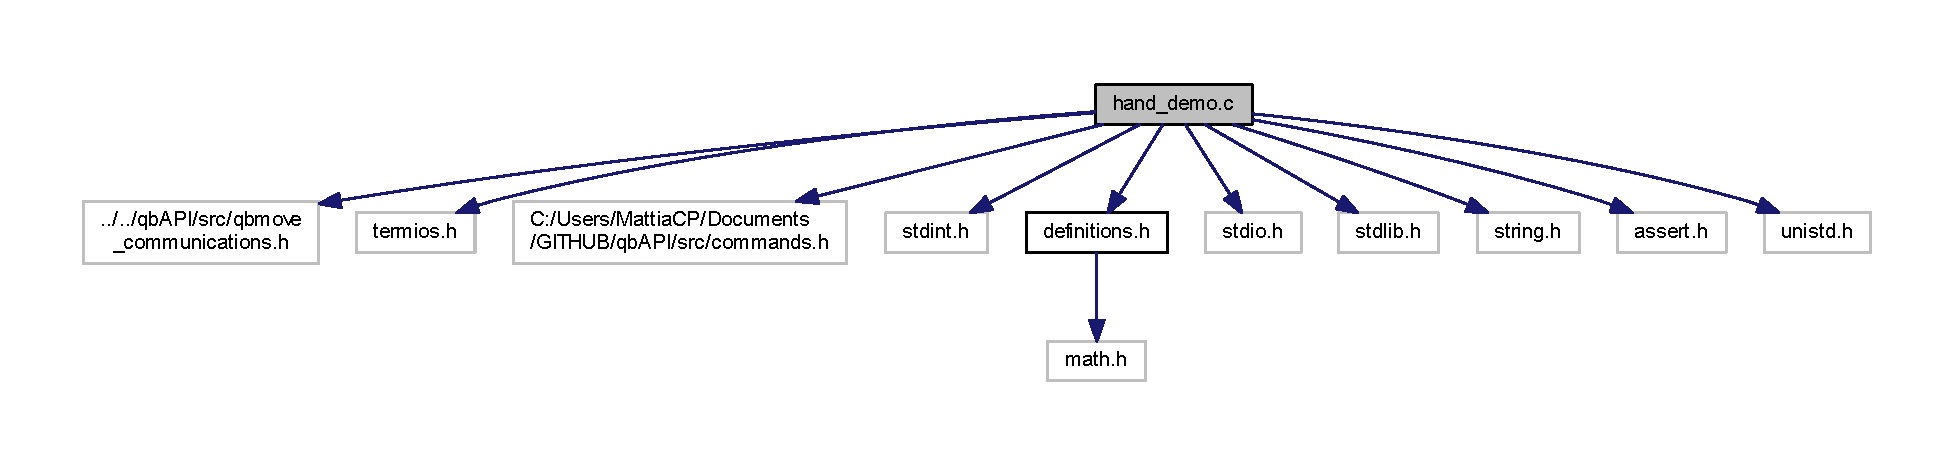
\includegraphics[width=350pt]{hand__demo_8c__incl}
\end{center}
\end{figure}
\subsection*{Functions}
\begin{DoxyCompactItemize}
\item 
\mbox{\label{hand__demo_8c_a4347eeebb915c2bd627acfbe8cda5bb9}} 
int {\bfseries port\+\_\+selection} (char $\ast$)
\item 
\mbox{\label{hand__demo_8c_a61a603d6ab622032ccf84775af74e960}} 
int {\bfseries open\+\_\+port} (char $\ast$)
\item 
\mbox{\label{hand__demo_8c_a432357bee330d9aac22de4131c290736}} 
int {\bfseries hand\+\_\+move} ()
\item 
\mbox{\label{hand__demo_8c_a005a3a684f8bd16cf4995c987f203c79}} 
void {\bfseries set\+\_\+input} (short int)
\item 
\mbox{\label{hand__demo_8c_a23b249b7c8456732056e88aa66bc2d30}} 
void {\bfseries get\+\_\+input} (short int $\ast$)
\item 
\mbox{\label{hand__demo_8c_a08bb75e02d6a2ded2201f0ad8f4af35e}} 
void {\bfseries print\+\_\+current} ()
\item 
\mbox{\label{hand__demo_8c_a3c04138a5bfe5d72780bb7e82a18e627}} 
int {\bfseries main} (int argc, char $\ast$$\ast$argv)
\end{DoxyCompactItemize}
\subsection*{Variables}
\begin{DoxyCompactItemize}
\item 
\mbox{\label{hand__demo_8c_accfd0301c469314772cc651ec198d492}} 
int {\bfseries device\+\_\+id}
\item 
\mbox{\label{hand__demo_8c_a92153f4b70cd8ba4e9b502ccff8d28bf}} 
comm\+\_\+settings {\bfseries comm\+\_\+settings\+\_\+t}
\item 
\mbox{\label{hand__demo_8c_a08c3ee234f2235f48480efc1225c50b3}} 
const int {\bfseries def\+\_\+inc} = 100
\end{DoxyCompactItemize}


\subsection{Detailed Description}
Demonstration file. 

\begin{DoxyAuthor}{Author}
{\itshape Centro \char`\"{}\+E.\+Piaggio\char`\"{}} 
\end{DoxyAuthor}
\begin{DoxyCopyright}{Copyright}
(C) 2012-\/2016 qbrobotics. All rights reserved. 

(C) 2017 Centro \char`\"{}\+E.\+Piaggio\char`\"{}. All rights reserved.
\end{DoxyCopyright}
With this file is possible to see a brief demonstration of terminal device opening and closing. 
\section{qbadmin.\+c File Reference}
\label{qbadmin_8c}\index{qbadmin.\+c@{qbadmin.\+c}}


Command line tools file.  


{\ttfamily \#include \char`\"{}../../qb\+A\+P\+I/src/qbmove\+\_\+communications.\+h\char`\"{}}\newline
{\ttfamily \#include \char`\"{}definitions.\+h\char`\"{}}\newline
{\ttfamily \#include $<$stdio.\+h$>$}\newline
{\ttfamily \#include $<$stdint.\+h$>$}\newline
{\ttfamily \#include $<$stdlib.\+h$>$}\newline
{\ttfamily \#include $<$unistd.\+h$>$}\newline
{\ttfamily \#include $<$getopt.\+h$>$}\newline
{\ttfamily \#include $<$string.\+h$>$}\newline
{\ttfamily \#include $<$sys/time.\+h$>$}\newline
{\ttfamily \#include $<$math.\+h$>$}\newline
{\ttfamily \#include $<$signal.\+h$>$}\newline
{\ttfamily \#include $<$assert.\+h$>$}\newline
Include dependency graph for qbadmin.\+c\+:\nopagebreak
\begin{figure}[H]
\begin{center}
\leavevmode
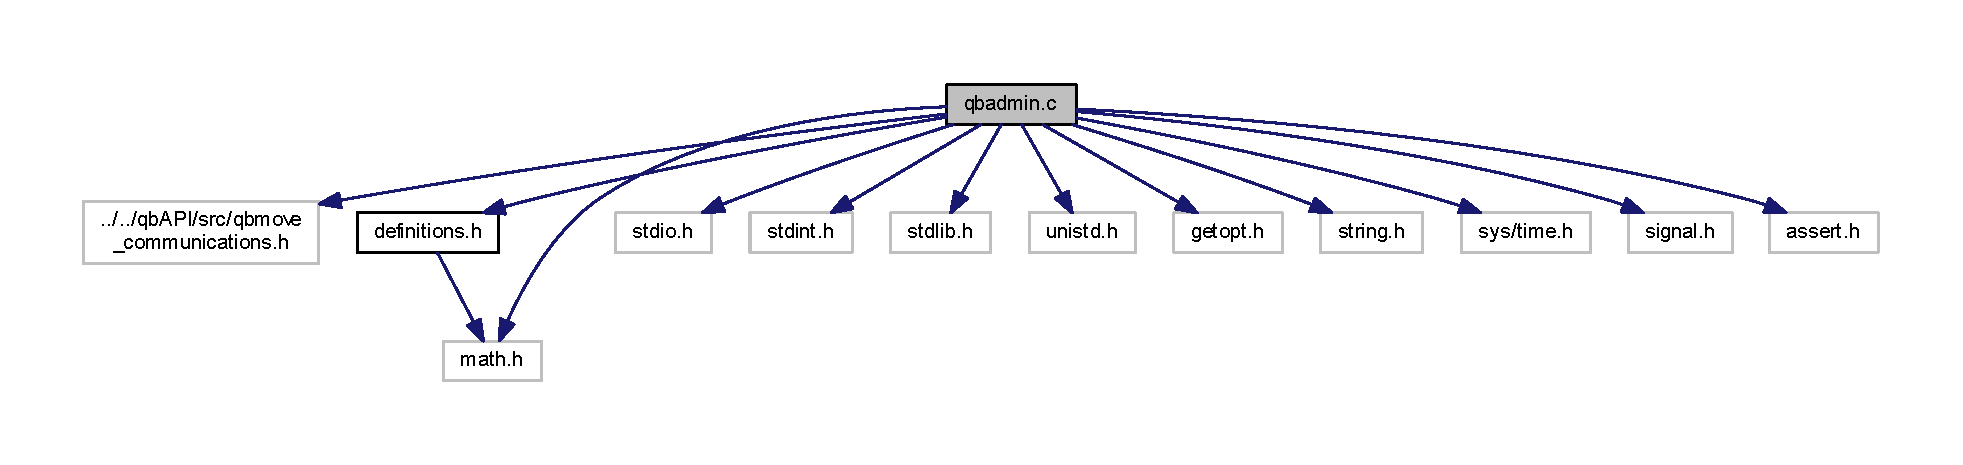
\includegraphics[width=350pt]{qbadmin_8c__incl}
\end{center}
\end{figure}
\subsection*{Data Structures}
\begin{DoxyCompactItemize}
\item 
struct \textbf{ global\+\_\+args}
\item 
struct \textbf{ position}
\end{DoxyCompactItemize}
\subsection*{Functions}
\begin{DoxyCompactItemize}
\item 
\mbox{\label{qbadmin_8c_abe553924eef0ba8079dc745caf1f348c}} 
int {\bfseries open\+\_\+port} ()
\item 
\mbox{\label{qbadmin_8c_a3939d4ef4a0e2be02b1eb9e1994ec985}} 
int {\bfseries port\+\_\+selection} ()
\item 
\mbox{\label{qbadmin_8c_a22b6aac07ec93fb920cc09b13175fa20}} 
int {\bfseries polling} ()
\item 
void \textbf{ display\+\_\+usage} (void)
\item 
float $\ast$$\ast$ \textbf{ file\+\_\+parser} (char $\ast$, int $\ast$, int $\ast$)
\item 
void \textbf{ int\+\_\+handler} (int sig)
\item 
void \textbf{ int\+\_\+handler\+\_\+2} (int sig)
\item 
void \textbf{ int\+\_\+handler\+\_\+3} (int sig)
\item 
int \textbf{ baudrate\+\_\+reader} ()
\item 
\mbox{\label{qbadmin_8c_abab28310fbbbcecb4658ce38e10ae89a}} 
int {\bfseries baudrate\+\_\+writer} (const int)
\item 
int \textbf{ main} (int argc, char $\ast$$\ast$argv)
\end{DoxyCompactItemize}
\subsection*{Variables}
\begin{DoxyCompactItemize}
\item 
static const struct option {\bfseries long\+Opts} [$\,$]
\item 
\mbox{\label{qbadmin_8c_a1b7271ddd60c22960c39ae6caf4d5254}} 
static const char $\ast$ {\bfseries opt\+String} = \char`\"{}s\+:adgptvh?f\+:ljqxzkycbe\+:uoi\+W\+:\+P\+B\+:\char`\"{}
\item 
\mbox{\label{qbadmin_8c_ac8e0866643ba994eff3e2fa3203885e0}} 
struct \textbf{ global\+\_\+args} {\bfseries global\+\_\+args}
\item 
\mbox{\label{qbadmin_8c_a821afb7ce4f1050e40bf615da3259a67}} 
struct \textbf{ position} {\bfseries p1}
\item 
\mbox{\label{qbadmin_8c_aeb1c5de60c0abd963c4b508d9f4c3cb1}} 
struct \textbf{ position} {\bfseries p2}
\item 
\mbox{\label{qbadmin_8c_a761d62937db066110a8f3e1479e8c404}} 
uint8\+\_\+t {\bfseries resolution} [4]
\item 
\mbox{\label{qbadmin_8c_a6baa346e44f4c2158d2be4f9b77b8203}} 
int {\bfseries ret}
\item 
\mbox{\label{qbadmin_8c_abf8643fca8c83efc67b50d0f2ecc8534}} 
int {\bfseries aux\+\_\+int}
\item 
\mbox{\label{qbadmin_8c_ae80455d5ff9aa4415b211f9842cb885e}} 
comm\+\_\+settings {\bfseries comm\+\_\+settings\+\_\+1}
\end{DoxyCompactItemize}


\subsection{Detailed Description}
Command line tools file. 

\begin{DoxyAuthor}{Author}
{\itshape Centro \char`\"{}\+E.\+Piaggio\char`\"{}} 
\end{DoxyAuthor}
\begin{DoxyCopyright}{Copyright}
(C) 2012-\/2016 qbrobotics. All rights reserved. 

(C) 2017 Centro \char`\"{}\+E.\+Piaggio\char`\"{}. All rights reserved.
\end{DoxyCopyright}
With this file is possible to command a terminal device. 

\subsection{Function Documentation}
\mbox{\label{qbadmin_8c_a872d84bb02f7d8f4617246f0c6d37c43}} 
\index{qbadmin.\+c@{qbadmin.\+c}!baudrate\+\_\+reader@{baudrate\+\_\+reader}}
\index{baudrate\+\_\+reader@{baudrate\+\_\+reader}!qbadmin.\+c@{qbadmin.\+c}}
\subsubsection{baudrate\+\_\+reader()}
{\footnotesize\ttfamily int baudrate\+\_\+reader (\begin{DoxyParamCaption}{ }\end{DoxyParamCaption})}

Baudrate functions \mbox{\label{qbadmin_8c_acf5088e61b616f77674f62a9ba3b86b7}} 
\index{qbadmin.\+c@{qbadmin.\+c}!display\+\_\+usage@{display\+\_\+usage}}
\index{display\+\_\+usage@{display\+\_\+usage}!qbadmin.\+c@{qbadmin.\+c}}
\subsubsection{display\+\_\+usage()}
{\footnotesize\ttfamily void display\+\_\+usage (\begin{DoxyParamCaption}\item[{void}]{ }\end{DoxyParamCaption})}

Display program usage, and exit. \mbox{\label{qbadmin_8c_a98a5d602fbf649e7f9e8f851cb757f71}} 
\index{qbadmin.\+c@{qbadmin.\+c}!file\+\_\+parser@{file\+\_\+parser}}
\index{file\+\_\+parser@{file\+\_\+parser}!qbadmin.\+c@{qbadmin.\+c}}
\subsubsection{file\+\_\+parser()}
{\footnotesize\ttfamily float $\ast$$\ast$ file\+\_\+parser (\begin{DoxyParamCaption}\item[{char $\ast$}]{filename,  }\item[{int $\ast$}]{deltat,  }\item[{int $\ast$}]{num\+\_\+values }\end{DoxyParamCaption})}

Parse csv input file with values to be sent to the motors

Parse C\+SV file and return a pointer to a matrix of float dinamically allocated. Remember to use free(pointer) in the caller \mbox{\label{qbadmin_8c_aa2bbc30ab4adea656f93d184270b0463}} 
\index{qbadmin.\+c@{qbadmin.\+c}!int\+\_\+handler@{int\+\_\+handler}}
\index{int\+\_\+handler@{int\+\_\+handler}!qbadmin.\+c@{qbadmin.\+c}}
\subsubsection{int\+\_\+handler()}
{\footnotesize\ttfamily void int\+\_\+handler (\begin{DoxyParamCaption}\item[{int}]{sig }\end{DoxyParamCaption})}

C\+T\+R\+L-\/c handler 1

handle C\+T\+R\+L-\/C interruption 1 \mbox{\label{qbadmin_8c_aaa3f1dc84f95d8979c957bb2d9c6df18}} 
\index{qbadmin.\+c@{qbadmin.\+c}!int\+\_\+handler\+\_\+2@{int\+\_\+handler\+\_\+2}}
\index{int\+\_\+handler\+\_\+2@{int\+\_\+handler\+\_\+2}!qbadmin.\+c@{qbadmin.\+c}}
\subsubsection{int\+\_\+handler\+\_\+2()}
{\footnotesize\ttfamily void int\+\_\+handler\+\_\+2 (\begin{DoxyParamCaption}\item[{int}]{sig }\end{DoxyParamCaption})}

C\+T\+R\+L-\/c handler 2

handle C\+T\+R\+L-\/C interruption 2 \mbox{\label{qbadmin_8c_affb492a4714b7e7b8047971581fd9aab}} 
\index{qbadmin.\+c@{qbadmin.\+c}!int\+\_\+handler\+\_\+3@{int\+\_\+handler\+\_\+3}}
\index{int\+\_\+handler\+\_\+3@{int\+\_\+handler\+\_\+3}!qbadmin.\+c@{qbadmin.\+c}}
\subsubsection{int\+\_\+handler\+\_\+3()}
{\footnotesize\ttfamily void int\+\_\+handler\+\_\+3 (\begin{DoxyParamCaption}\item[{int}]{sig }\end{DoxyParamCaption})}

C\+T\+R\+L-\/c handler 3

Handles the ctrl+c interruption to save the emg sensors measurements into a file \mbox{\label{qbadmin_8c_a3c04138a5bfe5d72780bb7e82a18e627}} 
\index{qbadmin.\+c@{qbadmin.\+c}!main@{main}}
\index{main@{main}!qbadmin.\+c@{qbadmin.\+c}}
\subsubsection{main()}
{\footnotesize\ttfamily int main (\begin{DoxyParamCaption}\item[{int}]{argc,  }\item[{char $\ast$$\ast$}]{argv }\end{DoxyParamCaption})}

main loop 

\subsection{Variable Documentation}
\mbox{\label{qbadmin_8c_a091f2d9683d6ef802780b360f66bad67}} 
\index{qbadmin.\+c@{qbadmin.\+c}!long\+Opts@{long\+Opts}}
\index{long\+Opts@{long\+Opts}!qbadmin.\+c@{qbadmin.\+c}}
\subsubsection{long\+Opts}
{\footnotesize\ttfamily const struct option long\+Opts[$\,$]\hspace{0.3cm}{\ttfamily [static]}}

{\bfseries Initial value\+:}
\begin{DoxyCode}
= \{
    \{ \textcolor{stringliteral}{"set\_inputs"}, required\_argument, NULL, \textcolor{charliteral}{'s'} \},
    \{ \textcolor{stringliteral}{"get\_measurements"}, no\_argument, NULL, \textcolor{charliteral}{'g'} \},
    \{ \textcolor{stringliteral}{"activate"}, no\_argument, NULL, \textcolor{charliteral}{'a'} \},
    \{ \textcolor{stringliteral}{"deactivate"}, no\_argument, NULL, \textcolor{charliteral}{'d'} \},
    \{ \textcolor{stringliteral}{"ping"}, no\_argument, NULL, \textcolor{charliteral}{'p'} \},
    \{ \textcolor{stringliteral}{"serial\_port"}, no\_argument, NULL, \textcolor{charliteral}{'t'} \},
    \{ \textcolor{stringliteral}{"verbose"}, no\_argument, NULL, \textcolor{charliteral}{'v'} \},
    \{ \textcolor{stringliteral}{"help"}, no\_argument, NULL, \textcolor{charliteral}{'h'} \},
    \{ \textcolor{stringliteral}{"file"}, required\_argument, NULL, \textcolor{charliteral}{'f'}\},
    \{ \textcolor{stringliteral}{"log"}, no\_argument, NULL, \textcolor{charliteral}{'l'}\},
    \{ \textcolor{stringliteral}{"get\_emg"}, no\_argument, NULL, \textcolor{charliteral}{'q'}\},
    \{ \textcolor{stringliteral}{"set\_zeros"}, no\_argument, NULL, \textcolor{charliteral}{'z'}\},
    \{ \textcolor{stringliteral}{"use\_gen\_sin"}, no\_argument, NULL, \textcolor{charliteral}{'y'}\},
    \{ \textcolor{stringliteral}{"get\_currents"}, no\_argument, NULL, \textcolor{charliteral}{'c'}\},
    \{ \textcolor{stringliteral}{"calibration"}, no\_argument, NULL, \textcolor{charliteral}{'k'}\},
    \{ \textcolor{stringliteral}{"bootloader"}, no\_argument, NULL, \textcolor{charliteral}{'b'}\},
    \{ \textcolor{stringliteral}{"joystick"}, no\_argument, NULL, \textcolor{charliteral}{'j'}\},
    \{ \textcolor{stringliteral}{"external drive"}, no\_argument, NULL, \textcolor{charliteral}{'x'}\},
    \{ \textcolor{stringliteral}{"set\_pos\_stiff"}, required\_argument, NULL, \textcolor{charliteral}{'e'}\},
    \{ \textcolor{stringliteral}{"get\_velocities"}, no\_argument, NULL, \textcolor{charliteral}{'i'}\},
    \{ \textcolor{stringliteral}{"get\_accelerations"}, no\_argument, NULL, \textcolor{charliteral}{'o'}\},
    \{ \textcolor{stringliteral}{"set\_cuff\_inputs"}, no\_argument, NULL, \textcolor{charliteral}{'u'}\},
   
    \{ \textcolor{stringliteral}{"baudrate"}, required\_argument, NULL, \textcolor{charliteral}{'B'}\},
    \{ \textcolor{stringliteral}{"set\_watchdog"}, required\_argument, NULL, \textcolor{charliteral}{'W'}\},
    \{ \textcolor{stringliteral}{"polling"}, no\_argument, NULL, \textcolor{charliteral}{'P'}\},
    \{ NULL, no\_argument, NULL, 0 \}
\}
\end{DoxyCode}

\section{qbmove\+\_\+backup.\+c File Reference}
\label{qbmove__backup_8c}\index{qbmove\+\_\+backup.\+c@{qbmove\+\_\+backup.\+c}}


Command line tools file.  


{\ttfamily \#include \char`\"{}../../qb\+A\+P\+I/src/qbmove\+\_\+communications.\+h\char`\"{}}\newline
{\ttfamily \#include \char`\"{}definitions.\+h\char`\"{}}\newline
{\ttfamily \#include $<$stdio.\+h$>$}\newline
{\ttfamily \#include $<$stdlib.\+h$>$}\newline
{\ttfamily \#include $<$string.\+h$>$}\newline
{\ttfamily \#include $<$assert.\+h$>$}\newline
{\ttfamily \#include $<$unistd.\+h$>$}\newline
{\ttfamily \#include $<$termios.\+h$>$}\newline
Include dependency graph for qbmove\+\_\+backup.\+c\+:\nopagebreak
\begin{figure}[H]
\begin{center}
\leavevmode
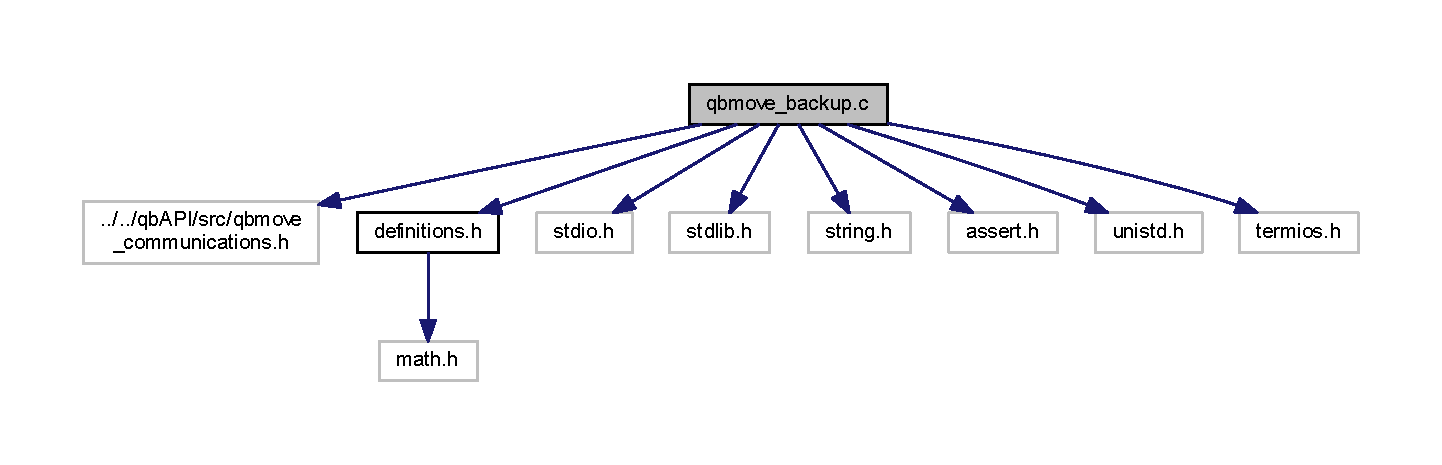
\includegraphics[width=350pt]{qbmove__backup_8c__incl}
\end{center}
\end{figure}
\subsection*{Functions}
\begin{DoxyCompactItemize}
\item 
\mbox{\label{qbmove__backup_8c_abe553924eef0ba8079dc745caf1f348c}} 
int {\bfseries open\+\_\+port} ()
\item 
\mbox{\label{qbmove__backup_8c_a19c7b4350b59e9273c8e5d38b2fee7e5}} 
int {\bfseries retrieve\+\_\+id} ()
\item 
\mbox{\label{qbmove__backup_8c_a820b26a1bfda44d50dcc4f87ec4b15e4}} 
int {\bfseries retrieve\+\_\+serial} ()
\item 
\mbox{\label{qbmove__backup_8c_acdbd97da27f51d67ecda3406dbe99b2e}} 
int {\bfseries retrieve\+\_\+offsets} ()
\item 
\mbox{\label{qbmove__backup_8c_a0b13dd1f535e14e1c234db426fdea510}} 
int {\bfseries read\+\_\+conf\+\_\+file} ()
\item 
\mbox{\label{qbmove__backup_8c_a67dbcb6dbe01df19e9379c9ed2204664}} 
int {\bfseries create\+\_\+file} ()
\item 
\mbox{\label{qbmove__backup_8c_a3221e1b236b178ebbb7cd09f7daf1842}} 
int {\bfseries write\+\_\+file} ()
\item 
\mbox{\label{qbmove__backup_8c_a327b46c721e061a90dec276552bdf79e}} 
int {\bfseries close\+\_\+file} ()
\item 
\mbox{\label{qbmove__backup_8c_ae66f6b31b5ad750f1fe042a706a4e3d4}} 
int {\bfseries main} ()
\end{DoxyCompactItemize}
\subsection*{Variables}
\begin{DoxyCompactItemize}
\item 
\mbox{\label{qbmove__backup_8c_accfd0301c469314772cc651ec198d492}} 
int {\bfseries device\+\_\+id}
\item 
\mbox{\label{qbmove__backup_8c_a5731872dfb5c314591bb61e35965e6cf}} 
char {\bfseries port} [255]
\item 
\mbox{\label{qbmove__backup_8c_ac04a6014404850aed62b804baff0748d}} 
char $\ast$ {\bfseries serial}
\item 
\mbox{\label{qbmove__backup_8c_a92153f4b70cd8ba4e9b502ccff8d28bf}} 
comm\+\_\+settings {\bfseries comm\+\_\+settings\+\_\+t}
\item 
\mbox{\label{qbmove__backup_8c_ac4e537e89adb6a44540bfef08b05d830}} 
short int {\bfseries offsets} [4]
\item 
\mbox{\label{qbmove__backup_8c_a2937a41bde0307e87626b85452766f89}} 
F\+I\+LE $\ast$ {\bfseries filep}
\item 
\mbox{\label{qbmove__backup_8c_ab0f61beb42e398815e77fd178651e333}} 
char {\bfseries backup\+\_\+folder} [512]
\item 
\mbox{\label{qbmove__backup_8c_a6fb6cb9ef16365b3861e2a813ad20037}} 
uint8\+\_\+t {\bfseries aux\+\_\+string} [2000]
\item 
\mbox{\label{qbmove__backup_8c_a088e92720e16f558a03834f4f43495a3}} 
int {\bfseries sensor\+\_\+num} = 0
\item 
\mbox{\label{qbmove__backup_8c_a390d0e64ffcfcf74f04fb0c4ee62970c}} 
short int {\bfseries temp\+\_\+meas} [4]
\end{DoxyCompactItemize}


\subsection{Detailed Description}
Command line tools file. 

\begin{DoxyAuthor}{Author}
{\itshape Centro \char`\"{}\+E.\+Piaggio\char`\"{}} 
\end{DoxyAuthor}
\begin{DoxyCopyright}{Copyright}
(C) 2012-\/2016 qbrobotics. All rights reserved. 

(C) 2017 Centro \char`\"{}\+E.\+Piaggio\char`\"{}. All rights reserved. 
\end{DoxyCopyright}

\section{qbmove\+\_\+init.\+c File Reference}
\label{qbmove__init_8c}\index{qbmove\+\_\+init.\+c@{qbmove\+\_\+init.\+c}}


Command line tools file.  


{\ttfamily \#include \char`\"{}../../qb\+A\+P\+I/src/qbmove\+\_\+communications.\+h\char`\"{}}\newline
{\ttfamily \#include \char`\"{}definitions.\+h\char`\"{}}\newline
{\ttfamily \#include $<$stdio.\+h$>$}\newline
{\ttfamily \#include $<$stdlib.\+h$>$}\newline
{\ttfamily \#include $<$string.\+h$>$}\newline
{\ttfamily \#include $<$assert.\+h$>$}\newline
{\ttfamily \#include $<$unistd.\+h$>$}\newline
{\ttfamily \#include $<$termios.\+h$>$}\newline
Include dependency graph for qbmove\+\_\+init.\+c\+:\nopagebreak
\begin{figure}[H]
\begin{center}
\leavevmode
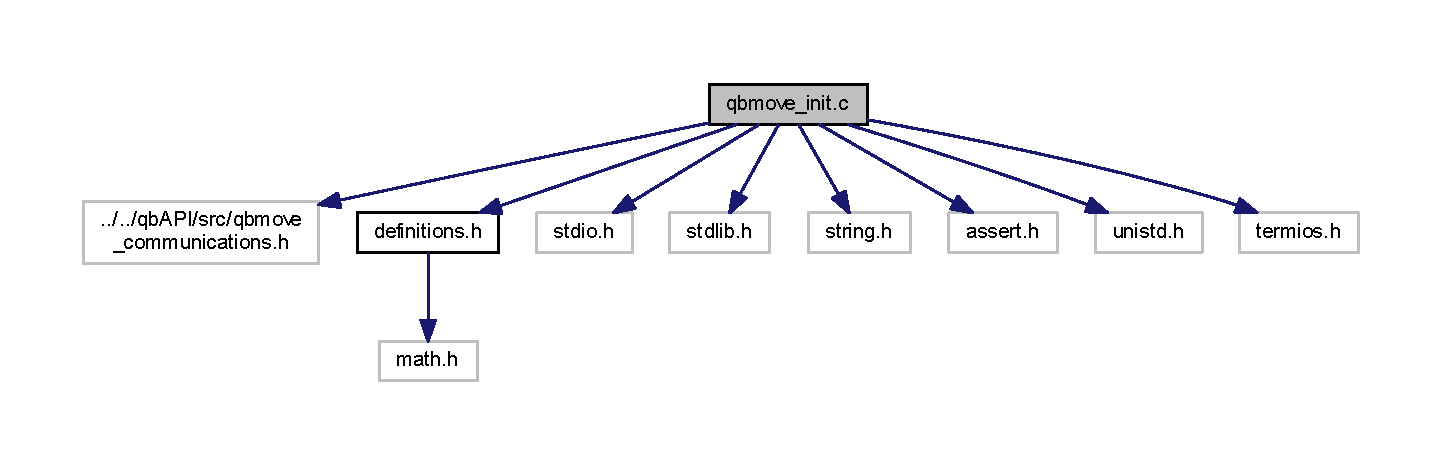
\includegraphics[width=350pt]{qbmove__init_8c__incl}
\end{center}
\end{figure}
\subsection*{Functions}
\begin{DoxyCompactItemize}
\item 
\mbox{\label{qbmove__init_8c_a44a4c36b1ed6edb012d9274fff39b156}} 
int {\bfseries mode\+\_\+selection} ()
\item 
\mbox{\label{qbmove__init_8c_a4347eeebb915c2bd627acfbe8cda5bb9}} 
int {\bfseries port\+\_\+selection} (char $\ast$)
\item 
\mbox{\label{qbmove__init_8c_a61a603d6ab622032ccf84775af74e960}} 
int {\bfseries open\+\_\+port} (char $\ast$)
\item 
\mbox{\label{qbmove__init_8c_ae0277117c43ff0ef7a3d500b96b003dd}} 
int {\bfseries init\+\_\+params} ()
\item 
\mbox{\label{qbmove__init_8c_a9f6588e3ddc3b88a01e5a0b4aa69079a}} 
int {\bfseries change\+\_\+id} ()
\item 
\mbox{\label{qbmove__init_8c_a8885d811c76fcef106bcb8260f8ae104}} 
int {\bfseries set\+\_\+resolution} (int)
\item 
\mbox{\label{qbmove__init_8c_ae95df945f6585dd892b8db7f3b9d48c5}} 
int {\bfseries set\+\_\+pid\+\_\+parameters} ()
\item 
\mbox{\label{qbmove__init_8c_a6070a0e69179adfda4f304f3ed7fbae7}} 
int {\bfseries adjust\+\_\+zeros} ()
\item 
\mbox{\label{qbmove__init_8c_a132b1b4c75e319d8d64a46b357857d04}} 
int {\bfseries get\+\_\+info} ()
\item 
\mbox{\label{qbmove__init_8c_ac8da963855e09bf929c085486f4a3b47}} 
int {\bfseries test} ()
\item 
\mbox{\label{qbmove__init_8c_a31a926c8b1f1d3abbde649bc34133547}} 
int {\bfseries backup} ()
\item 
\mbox{\label{qbmove__init_8c_aa78cef14864eb28be4f47d1ebf0e29f1}} 
int {\bfseries calibrate} ()
\item 
\mbox{\label{qbmove__init_8c_a3c04138a5bfe5d72780bb7e82a18e627}} 
int {\bfseries main} (int argc, char $\ast$$\ast$argv)
\end{DoxyCompactItemize}
\subsection*{Variables}
\begin{DoxyCompactItemize}
\item 
\mbox{\label{qbmove__init_8c_accfd0301c469314772cc651ec198d492}} 
int {\bfseries device\+\_\+id}
\item 
\mbox{\label{qbmove__init_8c_a92153f4b70cd8ba4e9b502ccff8d28bf}} 
comm\+\_\+settings {\bfseries comm\+\_\+settings\+\_\+t}
\end{DoxyCompactItemize}


\subsection{Detailed Description}
Command line tools file. 

\begin{DoxyAuthor}{Author}
{\itshape Centro \char`\"{}\+E.\+Piaggio\char`\"{}} 
\end{DoxyAuthor}
\begin{DoxyCopyright}{Copyright}
(C) 2012-\/2016 qbrobotics. All rights reserved. 

(C) 2017 Centro \char`\"{}\+E.\+Piaggio\char`\"{}. All rights reserved. 
\end{DoxyCopyright}

\section{qbmove\+\_\+pos\+\_\+stiff\+\_\+demo.\+c File Reference}
\label{qbmove__pos__stiff__demo_8c}\index{qbmove\+\_\+pos\+\_\+stiff\+\_\+demo.\+c@{qbmove\+\_\+pos\+\_\+stiff\+\_\+demo.\+c}}


Command line tools file.  


{\ttfamily \#include \char`\"{}../../qb\+A\+P\+I/src/qbmove\+\_\+communications.\+h\char`\"{}}\newline
{\ttfamily \#include \char`\"{}definitions.\+h\char`\"{}}\newline
{\ttfamily \#include $<$stdio.\+h$>$}\newline
{\ttfamily \#include $<$stdlib.\+h$>$}\newline
{\ttfamily \#include $<$string.\+h$>$}\newline
{\ttfamily \#include $<$assert.\+h$>$}\newline
{\ttfamily \#include $<$unistd.\+h$>$}\newline
{\ttfamily \#include $<$termios.\+h$>$}\newline
Include dependency graph for qbmove\+\_\+pos\+\_\+stiff\+\_\+demo.\+c\+:\nopagebreak
\begin{figure}[H]
\begin{center}
\leavevmode
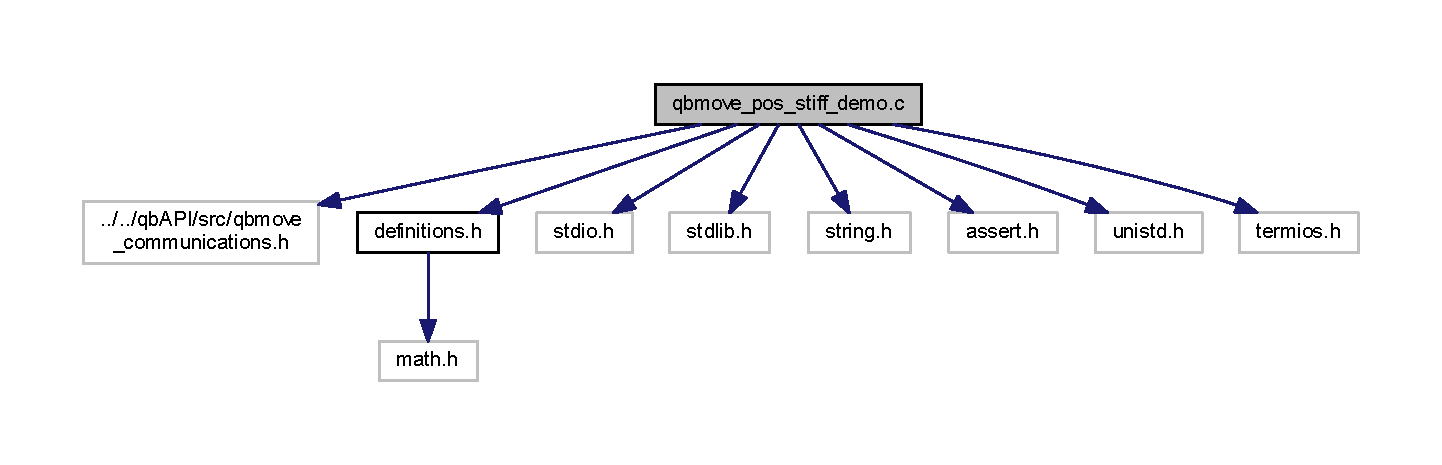
\includegraphics[width=350pt]{qbmove__pos__stiff__demo_8c__incl}
\end{center}
\end{figure}
\subsection*{Functions}
\begin{DoxyCompactItemize}
\item 
\mbox{\label{qbmove__pos__stiff__demo_8c_a4347eeebb915c2bd627acfbe8cda5bb9}} 
int {\bfseries port\+\_\+selection} (char $\ast$)
\item 
\mbox{\label{qbmove__pos__stiff__demo_8c_a61a603d6ab622032ccf84775af74e960}} 
int {\bfseries open\+\_\+port} (char $\ast$)
\item 
\mbox{\label{qbmove__pos__stiff__demo_8c_a04b53d850ce92eab6144de3aec004a74}} 
int {\bfseries pilot\+\_\+pos\+\_\+stiff} ()
\item 
\mbox{\label{qbmove__pos__stiff__demo_8c_a92250d16d1b963a26d5bafbcebfd53b6}} 
int {\bfseries set\+\_\+pos\+\_\+stiff} (short int $\ast$, short int $\ast$)
\item 
\mbox{\label{qbmove__pos__stiff__demo_8c_a3c04138a5bfe5d72780bb7e82a18e627}} 
int {\bfseries main} (int argc, char $\ast$$\ast$argv)
\end{DoxyCompactItemize}
\subsection*{Variables}
\begin{DoxyCompactItemize}
\item 
\mbox{\label{qbmove__pos__stiff__demo_8c_accfd0301c469314772cc651ec198d492}} 
int {\bfseries device\+\_\+id}
\item 
\mbox{\label{qbmove__pos__stiff__demo_8c_a92153f4b70cd8ba4e9b502ccff8d28bf}} 
comm\+\_\+settings {\bfseries comm\+\_\+settings\+\_\+t}
\end{DoxyCompactItemize}


\subsection{Detailed Description}
Command line tools file. 

\begin{DoxyAuthor}{Author}
{\itshape Centro \char`\"{}\+E.\+Piaggio\char`\"{}} 
\end{DoxyAuthor}
\begin{DoxyCopyright}{Copyright}
(C) 2012-\/2016 qbrobotics. All rights reserved. 

(C) 2017 Centro \char`\"{}\+E.\+Piaggio\char`\"{}. All rights reserved. 
\end{DoxyCopyright}

\section{qbmove\+\_\+test.\+c File Reference}
\label{qbmove__test_8c}\index{qbmove\+\_\+test.\+c@{qbmove\+\_\+test.\+c}}


Command line tools file.  


{\ttfamily \#include \char`\"{}../../qb\+A\+P\+I/src/qbmove\+\_\+communications.\+h\char`\"{}}\newline
{\ttfamily \#include \char`\"{}definitions.\+h\char`\"{}}\newline
{\ttfamily \#include $<$getopt.\+h$>$}\newline
{\ttfamily \#include $<$stdio.\+h$>$}\newline
{\ttfamily \#include $<$stdlib.\+h$>$}\newline
{\ttfamily \#include $<$assert.\+h$>$}\newline
{\ttfamily \#include $<$unistd.\+h$>$}\newline
{\ttfamily \#include $<$signal.\+h$>$}\newline
Include dependency graph for qbmove\+\_\+test.\+c\+:\nopagebreak
\begin{figure}[H]
\begin{center}
\leavevmode
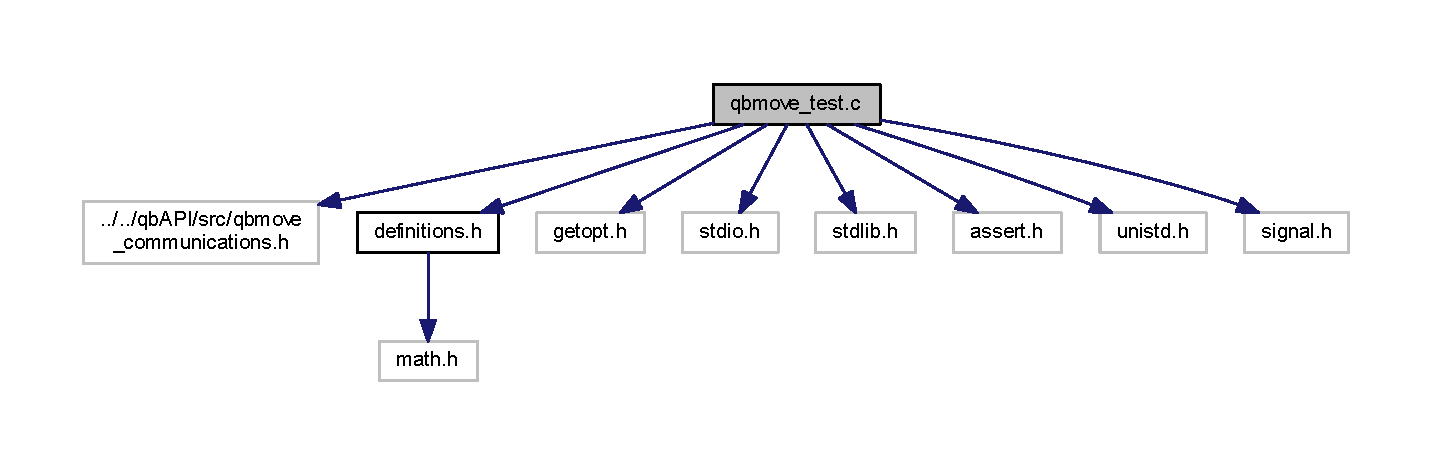
\includegraphics[width=350pt]{qbmove__test_8c__incl}
\end{center}
\end{figure}
\subsection*{Data Structures}
\begin{DoxyCompactItemize}
\item 
struct \textbf{ global\+\_\+var}
\end{DoxyCompactItemize}
\subsection*{Macros}
\begin{DoxyCompactItemize}
\item 
\mbox{\label{qbmove__test_8c_af24db198f37e801244816f9a63c126c3}} 
\#define {\bfseries R\+E\+P\+E\+T\+I\+T\+I\+O\+N\+\_\+\+P\+E\+R\+\_\+\+C\+Y\+C\+LE}~2
\item 
\mbox{\label{qbmove__test_8c_ac8d39f4363ce5ae611e4713705f13a04}} 
\#define {\bfseries B\+A\+T\+C\+H\+\_\+\+C\+Y\+C\+L\+ES}~5
\item 
\mbox{\label{qbmove__test_8c_a62249e384b997229a3e2ae74ade334e2}} 
\#define {\bfseries D\+E\+L\+AY}~1500000
\item 
\mbox{\label{qbmove__test_8c_a7a0ea3b7c06c69e1a12a585114ffb6b1}} 
\#define {\bfseries L\+I\+T\+T\+L\+E\+\_\+\+D\+E\+L\+AY}~5000
\item 
\mbox{\label{qbmove__test_8c_a5666ac5930c9f903698073ab1fa694f7}} 
\#define {\bfseries P\+A\+U\+SE}~30
\end{DoxyCompactItemize}
\subsection*{Functions}
\begin{DoxyCompactItemize}
\item 
\mbox{\label{qbmove__test_8c_ae5ad5cbeccaedc03a48d3c7eaa803e79}} 
void {\bfseries print\+\_\+usage} ()
\item 
\mbox{\label{qbmove__test_8c_abe553924eef0ba8079dc745caf1f348c}} 
int {\bfseries open\+\_\+port} ()
\item 
\mbox{\label{qbmove__test_8c_ab0dc12b72fe52d07687632cf2d31295d}} 
int {\bfseries cycle} ()
\item 
\mbox{\label{qbmove__test_8c_aa2bbc30ab4adea656f93d184270b0463}} 
void {\bfseries int\+\_\+handler} (int sig)
\item 
\mbox{\label{qbmove__test_8c_a3c04138a5bfe5d72780bb7e82a18e627}} 
int {\bfseries main} (int argc, char $\ast$$\ast$argv)
\end{DoxyCompactItemize}
\subsection*{Variables}
\begin{DoxyCompactItemize}
\item 
static const struct option {\bfseries long\+Opts} [$\,$]
\item 
\mbox{\label{qbmove__test_8c_a1b7271ddd60c22960c39ae6caf4d5254}} 
static const char $\ast$ {\bfseries opt\+String} = \char`\"{}t\+:r\+:\char`\"{}
\item 
\mbox{\label{qbmove__test_8c_a44064839969a9a8667c29d9f06dfd8c6}} 
struct \textbf{ global\+\_\+var} {\bfseries gv}
\item 
\mbox{\label{qbmove__test_8c_a92153f4b70cd8ba4e9b502ccff8d28bf}} 
comm\+\_\+settings {\bfseries comm\+\_\+settings\+\_\+t}
\item 
\mbox{\label{qbmove__test_8c_accfd0301c469314772cc651ec198d492}} 
int {\bfseries device\+\_\+id} = B\+R\+O\+A\+D\+C\+A\+S\+T\+\_\+\+ID
\end{DoxyCompactItemize}


\subsection{Detailed Description}
Command line tools file. 

\begin{DoxyAuthor}{Author}
{\itshape Centro \char`\"{}\+E.\+Piaggio\char`\"{}} 
\end{DoxyAuthor}
\begin{DoxyCopyright}{Copyright}
(C) 2012-\/2016 qbrobotics. All rights reserved. 

(C) 2017 Centro \char`\"{}\+E.\+Piaggio\char`\"{}. All rights reserved. 
\end{DoxyCopyright}


\subsection{Variable Documentation}
\mbox{\label{qbmove__test_8c_a091f2d9683d6ef802780b360f66bad67}} 
\index{qbmove\+\_\+test.\+c@{qbmove\+\_\+test.\+c}!long\+Opts@{long\+Opts}}
\index{long\+Opts@{long\+Opts}!qbmove\+\_\+test.\+c@{qbmove\+\_\+test.\+c}}
\subsubsection{long\+Opts}
{\footnotesize\ttfamily const struct option long\+Opts[$\,$]\hspace{0.3cm}{\ttfamily [static]}}

{\bfseries Initial value\+:}
\begin{DoxyCode}
= \{
    \{ \textcolor{stringliteral}{"set\_time"}, required\_argument, NULL, \textcolor{charliteral}{'t'}\},
    \{ \textcolor{stringliteral}{"set\_repetitions"}, required\_argument, NULL, \textcolor{charliteral}{'r'}\},
    \{ NULL, no\_argument, NULL, 0 \}
\}
\end{DoxyCode}

\section{qbparam.\+c File Reference}
\label{qbparam_8c}\index{qbparam.\+c@{qbparam.\+c}}


Command line tools file.  


{\ttfamily \#include \char`\"{}../../qb\+A\+P\+I/src/qbmove\+\_\+communications.\+h\char`\"{}}\newline
{\ttfamily \#include \char`\"{}definitions.\+h\char`\"{}}\newline
{\ttfamily \#include $<$assert.\+h$>$}\newline
{\ttfamily \#include $<$stdio.\+h$>$}\newline
{\ttfamily \#include $<$string.\+h$>$}\newline
{\ttfamily \#include $<$unistd.\+h$>$}\newline
{\ttfamily \#include $<$getopt.\+h$>$}\newline
{\ttfamily \#include $<$stdint.\+h$>$}\newline
Include dependency graph for qbparam.\+c\+:\nopagebreak
\begin{figure}[H]
\begin{center}
\leavevmode
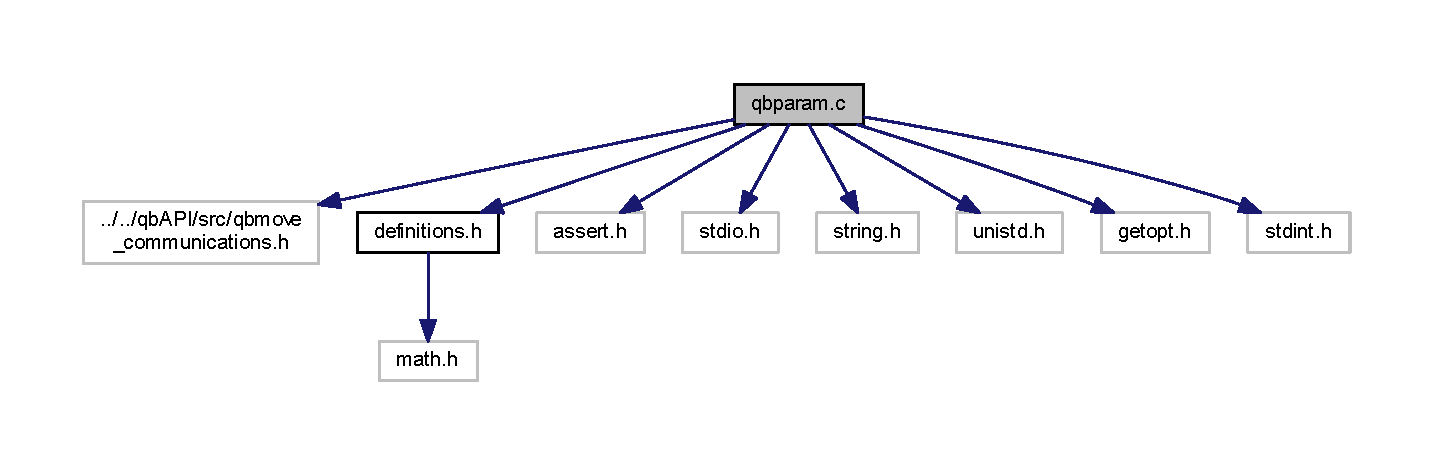
\includegraphics[width=350pt]{qbparam_8c__incl}
\end{center}
\end{figure}
\subsection*{Functions}
\begin{DoxyCompactItemize}
\item 
\mbox{\label{qbparam_8c_a3939d4ef4a0e2be02b1eb9e1994ec985}} 
int {\bfseries port\+\_\+selection} ()
\item 
\mbox{\label{qbparam_8c_abe553924eef0ba8079dc745caf1f348c}} 
int {\bfseries open\+\_\+port} ()
\item 
\mbox{\label{qbparam_8c_a564e2594b1cf22357d72b2e2cf7fdaf3}} 
int {\bfseries init\+Memory} ()
\item 
\mbox{\label{qbparam_8c_af9dce1973196a5934ee5ec20ea417324}} 
void {\bfseries print\+Main\+Menu} ()
\item 
\mbox{\label{qbparam_8c_a9c4b081f1e1ad60def15811c71a936f2}} 
void {\bfseries print\+Version} ()
\item 
\mbox{\label{qbparam_8c_aa78cef14864eb28be4f47d1ebf0e29f1}} 
int {\bfseries calibrate} ()
\item 
int \textbf{ baudrate\+\_\+reader} ()
\item 
\mbox{\label{qbparam_8c_a3c04138a5bfe5d72780bb7e82a18e627}} 
int {\bfseries main} (int argc, char $\ast$$\ast$argv)
\end{DoxyCompactItemize}
\subsection*{Variables}
\begin{DoxyCompactItemize}
\item 
\mbox{\label{qbparam_8c_a3c28322a1b5922f8c61d7cb3723b56b1}} 
char {\bfseries get\+\_\+or\+\_\+set}
\item 
\mbox{\label{qbparam_8c_a92153f4b70cd8ba4e9b502ccff8d28bf}} 
comm\+\_\+settings {\bfseries comm\+\_\+settings\+\_\+t}
\item 
\mbox{\label{qbparam_8c_aebf6cf4331fcc15f0d3ed0890e01a380}} 
uint8\+\_\+t {\bfseries device\+\_\+id} = B\+R\+O\+A\+D\+C\+A\+S\+T\+\_\+\+ID
\item 
\mbox{\label{qbparam_8c_a1b7271ddd60c22960c39ae6caf4d5254}} 
static const char $\ast$ {\bfseries opt\+String} = \char`\"{}\char`\"{}
\item 
static const struct option {\bfseries long\+Opts} [$\,$]
\end{DoxyCompactItemize}


\subsection{Detailed Description}
Command line tools file. 

\begin{DoxyAuthor}{Author}
{\itshape Centro \char`\"{}\+E.\+Piaggio\char`\"{}} 
\end{DoxyAuthor}
\begin{DoxyCopyright}{Copyright}
(C) 2012-\/2016 qbrobotics. All rights reserved. 

(C) 2017 Centro \char`\"{}\+E.\+Piaggio\char`\"{}. All rights reserved.
\end{DoxyCopyright}
With this file is possible to get or set firmware parameters. 

\subsection{Function Documentation}
\mbox{\label{qbparam_8c_a872d84bb02f7d8f4617246f0c6d37c43}} 
\index{qbparam.\+c@{qbparam.\+c}!baudrate\+\_\+reader@{baudrate\+\_\+reader}}
\index{baudrate\+\_\+reader@{baudrate\+\_\+reader}!qbparam.\+c@{qbparam.\+c}}
\subsubsection{baudrate\+\_\+reader()}
{\footnotesize\ttfamily int baudrate\+\_\+reader (\begin{DoxyParamCaption}{ }\end{DoxyParamCaption})}

Baudrate functions 

\subsection{Variable Documentation}
\mbox{\label{qbparam_8c_a091f2d9683d6ef802780b360f66bad67}} 
\index{qbparam.\+c@{qbparam.\+c}!long\+Opts@{long\+Opts}}
\index{long\+Opts@{long\+Opts}!qbparam.\+c@{qbparam.\+c}}
\subsubsection{long\+Opts}
{\footnotesize\ttfamily const struct option long\+Opts[$\,$]\hspace{0.3cm}{\ttfamily [static]}}

{\bfseries Initial value\+:}
\begin{DoxyCode}
= \{
    \{ \textcolor{stringliteral}{"id"}, required\_argument, NULL, 0 \},
    \{ NULL, no\_argument, NULL, 0\}
\}
\end{DoxyCode}

%--- End generated contents ---

% Index
\backmatter
\newpage
\phantomsection
\clearemptydoublepage
\addcontentsline{toc}{chapter}{Index}
\printindex

\end{document}
